% \documentclass[review]{cvpr}
\documentclass[final]{cvpr}

\usepackage{mathptmx}
\usepackage{epsfig}
\usepackage{graphicx}
\usepackage{amsmath}
\usepackage{amssymb}
\usepackage{subfig}

% Include other packages here, before hyperref.

% If you comment hyperref and then uncomment it, you should delete
% egpaper.aux before re-running latex.  (Or just hit 'q' on the first latex
% run, let it finish, and you should be clear).
\usepackage[pagebackref=true,breaklinks=true,colorlinks,bookmarks=false]{hyperref}

\def\cvprPaperID{****} % *** Enter the CVPR Paper ID here
\def\confYear{CVPR 2021}
%\setcounter{page}{4321} % For final version only
\pdfminorversion=7

\begin{document}

%%%%%%%%% TITLE
\title{Automated Camera Stabilization and Calibration \\for Intelligent Transportation Systems}

\author{Marcel Bruckner\\
% Informatics 6 - Chair of Robotics, Artificial Intelligence and Real-time Systems\\
% TUM Department of Informatics\\
Technische Universität München\\
Boltzmannstraße 15, 85748 Garching\\
{\tt\small marcel.bruckner@tum.de}
}

\maketitle

% !TEX root=./report.tex

\newcommand{\Providentia}{\emph{\href{https://innovation-mobility.com/}{Providentia++}} project \cite{kraemmer2020providentia}} 
\newcommand{\ITS}{Intelligent Transportation System}
\newcommand{\AD}{Autonomous Driving}
\newcommand{\HDmap}{HD map}
\newcommand{\HDmaps}{\HDmap{}s}
\newcommand{\Sc}{static scene (\ref{sec:dynamic_foreground_static_scene})}
\newcommand{\DigitalTwin}{Digital Twin (\ref{sec:digital_twin})}
\newcommand{\OD}{OpenDRIVE}

\newcommand{\hr}{\noindent\rule{\linewidth}{0.4pt}}

%%%%%%%%% ABSTRACT
%!TEX root = ../report.tex
\begin{abstract}

In the emerging field of Intelligent Transportation Systems one main challenge is the fusion of different sensor types.
To fuse the measurements exactly each sensor needs to be free from noise and calibrated accurately.
In this work we focus on two problems resulting from environmental influences on RGB cameras within the Providentia++~project.

First we propose an online vision-based pipeline to remove motion jitter from camera streams to dynamically stabilize the video feed.
We show that our approach based on visual features and an image space homographic transformation significantly stabilizes the frames regarding the optical flow as measure. 
By exemplary tracking objects and measuring their travelled pixel distance we show a substantial decrease of the jittery image motion. 

Second we propose an online Bundle Adjustment formulation based on the reprojection-error to statically calibrate single RBG-only cameras \wrt{} a high definition map and to mitigate drift of the intrinsic and extrinsic camera parameters over time.
By relaxing the minimization problem using a 1D-approximation of road signs we achieve high accuracy in the calibration of the cameras.
We show the minimal number of correspondences needed between the video stream and the map, the structure they have to exceed and give lower bounds on the remaining calibration errors. 

\end{abstract}


\keywords{
    Intelligent Transportation Systems,
    Computer Vision,
    Video Stabilization,
    Feature Detection,
    Feature Matching,
    Camera Calibration,
    Bundle Adjustment,
    Reprojection-error,
    Optimization,
    OpenDRIVE
}


%%%%%%%%% BODY TEXT
% !TEX root=./report.tex

\section{Introduction}

Within the \Providentia{}, a section of the highway A9 between Munich and Nuremberg was converted to a testing site for autonomous driving. 
As part of this, a large sensor network system has been set up along the highway to allow monitoring and steering of traffic as well as to improve the coordination between autonomous and traditional cars. 
The primary task of the intelligent transportation system (ITS) is to create a digital traffic twin that accurately represents the physical road situation in real-time. 
Based on this digital twin, the smart infrastructure can provide a far-reaching and comprehensive view to the drivers and autonomous vehicles in order to improve their situational awareness within the current traffic environment.

A key challenge of ITS lies in the reliable and accurate calibration of the different sensors.
The calibration is especially challenging when the sensor is subject to real-life disturbances like vibration of its mounting pole caused by wind or displacements due to temperature expansion.
In this work we focus on removing the noise introduced by these disturbances and its implications for the vision system built upon cameras mounted to gantry bridges.

We propose two computer vision-based approaches to tackle the environmental influences and to remove noise from the system.
The solved problems can be roughly grouped into problems concerning the dynamic stabilization of the video feed and the static calibration of the camera setup.

\paragraph{Dynamic Stabilization}
The cameras are constantly exposed to wind and vibrations from passing vehicles.
These influences propagate into the video stream and result in jittery motion of the images.
We propose a pipeline to counteract the shaky motions of the cameras using a digital image stabilization approach.
The approach is based on visual image features that are matched between the current and a stable reference frame. 
The feature matching is used to minimize the reprojection-error between the frames and results in a homographic transformation.
We use the transformation to align the static backgrounds of the frames, thus mitigating the real-world motion of the camera in image space.

\paragraph{Static Calibration}
We track and predict the real-world location of the vehicles in the test area to pass this information to the drivers and autonomous vehicles. 
To accurately predict the locations the system needs to be calibrated precisely towards a global reference frame. 
This is a time consuming process that often has to be done by hand. 
The cameras translational, rotational and intrinsic parameters decalibrate over time due to environmental influences on the mounting constructions and gantry bridges as well as from the natural wear of the materials.

Within the project high definition maps (HD maps) of the enclosed environment are used extensively. 
These HD maps offer approximations of the real-world positions of the highway lanes, the gantry bridges, objects like poles and permanent delineators and traffic signals like speed limits or exit markers.
We use this spatial information and a mapping from the objects to pixels in the video frame to solve a Bundle Adjustment (BA) problem by minimizing the reprojection-error.
We jointly optimize for the cameras intrinsic and extrinsic parameters as well as the real-world locations to recover the camera poses from the observations.

\paragraph{Code Repositories}
The code for the dynamic stabilization, static calibration and object position retrieval from the HD maps are accessible via two GitHub repositories: \url{https://github.com/Brucknem/GuidedResearch} and \url{https://github.com/Brucknem/OpenDRIVE}.

% !TEX root=./report.tex

\section{Terms and Definitions}
This section provides explanations of extensively used terms and definitions. 

\subsection{Dynamic foreground and \Sc{}}
\label{sec:dynamic_foreground_static_scene}
We group parts of the world seen by the cameras into the two groups of dynamic foreground and \Sc{}.
Dynamic foreground describes all pixels that represent objects that are meant to be moving, \eg{} vehicles on the roads.
On the other hand the \Sc{} are all pixels that are not dynamic foreground, \eg{} the road, guardrails or bridges.
\section{Related Work}
There are many ITS projects emerging \eg{} Koster \etal{} at the \emph{Testfeld für Autonomes und vernetztes Fahren in Niedersachsen} \cite{koster2017testfeld}. 
Also cooperative perception using infrastructure sensors is an emerging field \cite{arnold2020cooperative}.

None of the teams - to the best of our knowledge - provide in depth public information about their camera stabilization and calibration approaches.

In the \TAADBW{} (TAADBW) project multiple optical camera sensors are attached to large poles with overlapping fields of view.
They calibrate their cameras relative to a high-precision map and assume the calibration and the intrinsic camera parameters to be static during runtime. 
The team relies on an manual a-priori selection of visual landmarks and perform calibration at system startup.  
The team of the TAADBW estimate the extrinsic calibration with exact world position from the map by minimizing the squared distances between the visible landmarks and the respective projected objects.
The large overlaps in the fields of view in their setup allow a global optimization strategy. 
This is not feasible in our project due to the small overlaps in the fields of view between the cameras \cite{kraemmer2020providentia} and associating pixels within the multi-view setup is an inherently hard problem. 

Müller \etal{} \cite{laciMueller} present an approach based on a cooperative intelligent vehicle.
The vehicle moves through the scene and passes cooperative awareness messages from the vehicle to the infrastructure. 
This removes the need for overlapping fields of view completely and enables a fully automated and sensor-independent registration.
The team calibrates a multitude of different sensor types to the world frame and recovers their extrinsic parameters. 

Calibration between cameras and radar sensors has been solved previously by Schöller \etal{} within the \Providentia{}.
% !TEX root=./report.tex

\section{Approach}
In this paper we propose two algorithms to solve distinct problems that arise from real-world disturbances that act upon the ITS.

\subsection{Dynamic Stabilization}
\label{sec:dynamic_stabilization_approach}

\begin{figure}[t]
   \begin{center}
      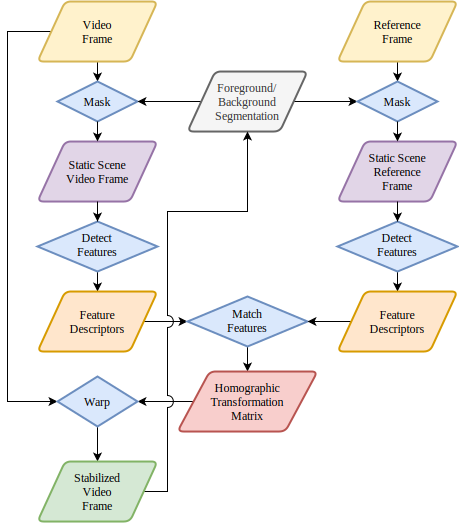
\includegraphics[width=0.8\linewidth]{diagrams/DynamicStabilization.pdf}
   \end{center}
   \caption{
      The proposed dynamic stabilization pipeline. 
      The input is the video and a stable reference frame.
      The frames are segmented into the foreground and background to extract the static scene.
      On the static scene visual features are detected and the feature descriptors are matched.
      We use the homographic transformation minimizing the reprojection-error based on the matching to warp the video frame.
      The stabilized frame is used to update the background segmentation mask.
       }
   \label{fig:dynamic_stabilization_algorithm}
\end{figure}

The camera sensors used in the project are mounted to gantry bridges spanning over the highway.
Environmental influences, \eg{} wind or vibrations from passing vehicles, bring the bridges into a swinging state that spreads onto the cameras. 
This unwanted real world movement propagates into the video feeds output by the cameras and introduces jittery motion in image space. 
We assume the cameras to be mostly static, thus we only face disturbances within a small range around the resting position.
Nonetheless, the small disturbances get amplified by the huge distances covered by the cameras and introduce substantial error.

To mitigate the noise added by the jittery motion we propose the pipeline displayed in \Cref{fig:dynamic_stabilization_algorithm} and explained in the following.

%%%%%%%%%%%%%%%%%%%%%%%%%%%%%%%%%%%%%%%%%%%%%%%%%%%%%%%%%%%%%%%%%%%%%%%%%%%%%%%%%%%%%%%%%%%%%%%%%%%%%%%%%%%%%%%%%%%%
%%%%%%%%%%%%%%%%%%%%%%%%%%%%%%%%%%%%%%%%%%%%%%%%%%%%%%%%%%%%%%%%%%%%%%%%%%%%%%%%%%%%%%%%%%%%%%%%%%%%%%%%%%%%%%%%%%%%
%%%%%%%%%%%%%%%%%%%%%%%%%%%%%%%%%%%%%%%%%%%%%%%%%%%%%%%%%%%%%%%%%%%%%%%%%%%%%%%%%%%%%%%%%%%%%%%%%%%%%%%%%%%%%%%%%%%%

\paragraph{Extract Static Background}
We stabilize the input frame by minimizing the reprojection-error between the video frame and the reference frame, thus aligning the images.
This alignment is based on the matching of features between the frames, whereas we do not align the moving vehicles, but only the static non-moving background, \eg{} the road, poles, guardrails and bridges.
We assume that the background does not move in the real world, thus aligning it during image warping ensures that the scene stays static and only the vehicles real movement is kept.
Hence, we extract the static background from the input frame and the stable reference frame using a background segmentation based on
the \emph{Improved Adaptive Gaussian Mixture Model for Background Subtraction} proposed by Zoran Zivkovic \etal{} \cite{zivkovic10.5555/1018428.1020644,zivkovic10.1016/j.patrec.2005.11.005,opencv_library}.

%%%%%%%%%%%%%%%%%%%%%%%%%%%%%%%%%%%%%%%%%%%%%%%%%%%%%%%%%%%%%%%%%%%%%%%%%%%%%%%%%%%%%%%%%%%%%%%%%%%%%%%%%%%%%%%%%%%%
%%%%%%%%%%%%%%%%%%%%%%%%%%%%%%%%%%%%%%%%%%%%%%%%%%%%%%%%%%%%%%%%%%%%%%%%%%%%%%%%%%%%%%%%%%%%%%%%%%%%%%%%%%%%%%%%%%%%
%%%%%%%%%%%%%%%%%%%%%%%%%%%%%%%%%%%%%%%%%%%%%%%%%%%%%%%%%%%%%%%%%%%%%%%%%%%%%%%%%%%%%%%%%%%%%%%%%%%%%%%%%%%%%%%%%%%%

\paragraph{Feature Detection}
\begin{figure}[t]
   \begin{center}
      \includegraphics[width=\linewidth]{images/feature_matching.png}
   \end{center}
   \caption{
      Left: The input frame. 
      Right: The stable reference frame.
      The colorful lines display the matching between image features. 
      The ends of the lines are the location of the features.
       }
   \label{fig:dynamic_stabilization_feature_matching}
\end{figure}

We search the static background for pixel locations that are prominent and depict specific patterns that are unique and can easily be compared.
The detected features describe the location based on different metrics, \eg{} the local image gradient, oriented histograms or haar-like features \cite{stork2001pattern}.
Kumar \etal{} \cite{kumar2014survey} give in depth descriptions of a multitude of feature detectors and descriptors.

We implemented the SURF \cite{bay10.1007/11744023_32} and ORB \cite{rublee6126544} feature detectors and descriptors and the Fast \cite{Ghahremani_2021} feature detector with FREAK \cite{alahi6247715} feature descriptors. The algorithmic implementation is included in the OpenCV library \cite{opencv_library}. 

%%%%%%%%%%%%%%%%%%%%%%%%%%%%%%%%%%%%%%%%%%%%%%%%%%%%%%%%%%%%%%%%%%%%%%%%%%%%%%%%%%%%%%%%%%%%%%%%%%%%%%%%%%%%%%%%%%%%
%%%%%%%%%%%%%%%%%%%%%%%%%%%%%%%%%%%%%%%%%%%%%%%%%%%%%%%%%%%%%%%%%%%%%%%%%%%%%%%%%%%%%%%%%%%%%%%%%%%%%%%%%%%%%%%%%%%%
%%%%%%%%%%%%%%%%%%%%%%%%%%%%%%%%%%%%%%%%%%%%%%%%%%%%%%%%%%%%%%%%%%%%%%%%%%%%%%%%%%%%%%%%%%%%%%%%%%%%%%%%%%%%%%%%%%%%

\paragraph{Feature Matching}
We compare the detected features from the input frame with the features from the stable reference frame.
A match is reported if the feature descriptors of two compared features surpass the Lowe's ratio test \cite{lowe10.1023/B:VISI.0000029664.99615.94} regarding some feature dependent metric \cite{kumar2014survey}.
These feature matches establish a spatial relationship in pixel space between the two frames.
\Cref{fig:dynamic_stabilization_feature_matching} displays an exemplary feature matching.

We estimate a homographic transformation $H$ that maps the homogeneous pixel locations $(x_i, y_i, 1)^T$ of the input frame to the matched pixel locations $(x'_i, y'_i, 1)^T$ in the stable reference frame.
We minimize the reprojection-error between the pixels so that for each match $i$ it holds
\begin{equation}
 z_i  * (x'_i, y'_i, 1)^T \sim H * (x_i, y_i, 1)^T
 \label{eq:dynamic_stabilization_homographic_transformation}
\end{equation}
where $z_i$ is the homogeneous component used in the perspective division. 
We use a RANSAC \cite{fischler1981random} based estimation procedure to robustify the minimization against outliers.

The algorithmic implementation is included in the OpenCV library \cite{opencv_library}.

%%%%%%%%%%%%%%%%%%%%%%%%%%%%%%%%%%%%%%%%%%%%%%%%%%%%%%%%%%%%%%%%%%%%%%%%%%%%%%%%%%%%%%%%%%%%%%%%%%%%%%%%%%%%%%%%%%%%
%%%%%%%%%%%%%%%%%%%%%%%%%%%%%%%%%%%%%%%%%%%%%%%%%%%%%%%%%%%%%%%%%%%%%%%%%%%%%%%%%%%%%%%%%%%%%%%%%%%%%%%%%%%%%%%%%%%%
%%%%%%%%%%%%%%%%%%%%%%%%%%%%%%%%%%%%%%%%%%%%%%%%%%%%%%%%%%%%%%%%%%%%%%%%%%%%%%%%%%%%%%%%%%%%%%%%%%%%%%%%%%%%%%%%%%%%

\paragraph{Image Alignment}
We use the found homographic transformation to warp the whole input frame, thus aligning the background of the frames.
As the keyframe is stable and does not change over time the current video frame is also stabilized.
The alignment minimizes the motion of the static background scene and leaves only the real expected movement of the vehicles.

%%%%%%%%%%%%%%%%%%%%%%%%%%%%%%%%%%%%%%%%%%%%%%%%%%%%%%%%%%%%%%%%%%%%%%%%%%%%%%%%%%%%%%%%%%%%%%%%%%%%%%%%%%%%%%%%%%%%
%%%%%%%%%%%%%%%%%%%%%%%%%%%%%%%%%%%%%%%%%%%%%%%%%%%%%%%%%%%%%%%%%%%%%%%%%%%%%%%%%%%%%%%%%%%%%%%%%%%%%%%%%%%%%%%%%%%%
%%%%%%%%%%%%%%%%%%%%%%%%%%%%%%%%%%%%%%%%%%%%%%%%%%%%%%%%%%%%%%%%%%%%%%%%%%%%%%%%%%%%%%%%%%%%%%%%%%%%%%%%%%%%%%%%%%%%

\paragraph{Upate of Background Segmentation}
We use the stabilized frame to update the segmentation of the foreground and background.
We assume the motion between frames to be relatively small, thus we use the segmentation of the stabilized frame for the next frame.
This reduces the search space for the feature detectors and prohibits matches between static scene and dynamic foreground objects. 
% Hence, the algorithm is robustified and speed up.

% !TEX root=./report.tex

\subsection{Static Calibration}
\label{sec:static_calibration_approach}

ITS are inherently dependent on the calibration of the different sensors. 
The system has to know the poses of the different sensors relative to some reference coordinate system to accurately measure the position of vehicles within the single sensor ranges and at the overlapping boundaries.

We propose a calibration procedure based on a Bundle Adjustment (BA) problem formulation.
We map visual landmarks in the video feed to their partially known world positions from high definition road maps (HD maps).
We recover the pose by jointly optimizing for the camera intrinsic and extrinsic parameters as well as the real world positions of the landmarks. 

%%%%%%%%%%%%%%%%%%%%%%%%%%%%%%%%%%%%%%%%%%%%%%%%%%%%%%%%%%%%%%%%%%%%%%%%%%%%%%%%%%%%%%%%%%%%%%%%%%%%%%%%%%%%%%%%%%%%%%%%%%%%%%%%%%%%%%%%%%%%%%%%%%%%%%%%%%%%%%%%%
%%%%%%%%%%%%%%%%%%%%%%%%%%%%%%%%%%%%%%%%%%%%%%%%%%%%%%%%%%%%%%%%%%%%%%%%%%%%%%%%%%%%%%%%%%%%%%%%%%%%%%%%%%%%%%%%%%%%%%%%%%%%%%%%%%%%%%%%%%%%%%%%%%%%%%%%%%%%%%%%%
%%%%%%%%%%%%%%%%%%%%%%%%%%%%%%%%%%%%%%%%%%%%%%%%%%%%%%%%%%%%%%%%%%%%%%%%%%%%%%%%%%%%%%%%%%%%%%%%%%%%%%%%%%%%%%%%%%%%%%%%%%%%%%%%%%%%%%%%%%%%%%%%%%%%%%%%%%%%%%%%%

\paragraph{Retrieve Objects from High Definition Maps}

In our project we use HD maps in the \OD{} standard format.
In this work we focus on the permanent delineator (PD) objects that are easily visible in the video feeds.

We extract the world position of the PDs using the mathematical operations defined in the \OD{} standard.
This gives us the the base origin point $o~=~(x, y, z)^T$ of the PDs in the Universal Transverse Mercator (UTM) projection \cite{langley1998utm,proj}. 
This point $o$ is the world position of the lower end of the PD where it touches the ground or another object.
Additionally, we retrieve a directional heading axis $d~=~(x, y, z)^T$ and the height $h$ of the PD.

\paragraph{1D Approximation of Objects}

In the original BA setting the optimization is done jointly over multiple cameras and observations, and the arising stereo vision problem is solved jointly for the 3D positions of the objects and the camera parameters.
For this system of equations to be solvable it requires multiple cameras from different viewing angles and large overlapping fields of view between the cameras.

In our project we have neither of requirements and calibrate each camera separately to the HD map.
We relax the BA problem by the 1D approximation of the PDs
\begin{equation}
S = \{o + \lambda * d: \quad \lambda \in [0, h]\}
\end{equation}
where $S$ is the set of points along its central axis between its base at $\lambda = 0$ and its top at $\lambda = h$.
This approximation allows for a joint optimization of their world positions and the camera intrinsic and extrinsic parameters.

\autoref{sec:static_calibration_number_points} derives a minimal number of points for the resulting system of equations to be solvable.

% The assumptions we made are: 
% \begin{itemize}
  % \item Objects are symmetric around their directional heading axis.
  % \item Projected pixels of the objects are also symmetric around the projected directional axis.
% \end{itemize}


%%%%%%%%%%%%%%%%%%%%%%%%%%%%%%%%%%%%%%%%%%%%%%%%%%%%%%%%%%%%%%%%%%%%%%%%%%%%%%%%%%%%%%%%%%%%%%%%%%%%%%%%%%%%%%%%%%%%%%%%%%%%%%%%%%%%%%%%%%%%%%%%%%%%%%%%%%%%%%%%%
%%%%%%%%%%%%%%%%%%%%%%%%%%%%%%%%%%%%%%%%%%%%%%%%%%%%%%%%%%%%%%%%%%%%%%%%%%%%%%%%%%%%%%%%%%%%%%%%%%%%%%%%%%%%%%%%%%%%%%%%%%%%%%%%%%%%%%%%%%%%%%%%%%%%%%%%%%%%%%%%%
%%%%%%%%%%%%%%%%%%%%%%%%%%%%%%%%%%%%%%%%%%%%%%%%%%%%%%%%%%%%%%%%%%%%%%%%%%%%%%%%%%%%%%%%%%%%%%%%%%%%%%%%%%%%%%%%%%%%%%%%%%%%%%%%%%%%%%%%%%%%%%%%%%%%%%%%%%%%%%%%%

\paragraph{Mapping Objects to Pixels}
\begin{figure}[t]
  \begin{center}
  % \fbox{\rule{0pt}{2in} \rule{0.9\linewidth}{0pt}}
     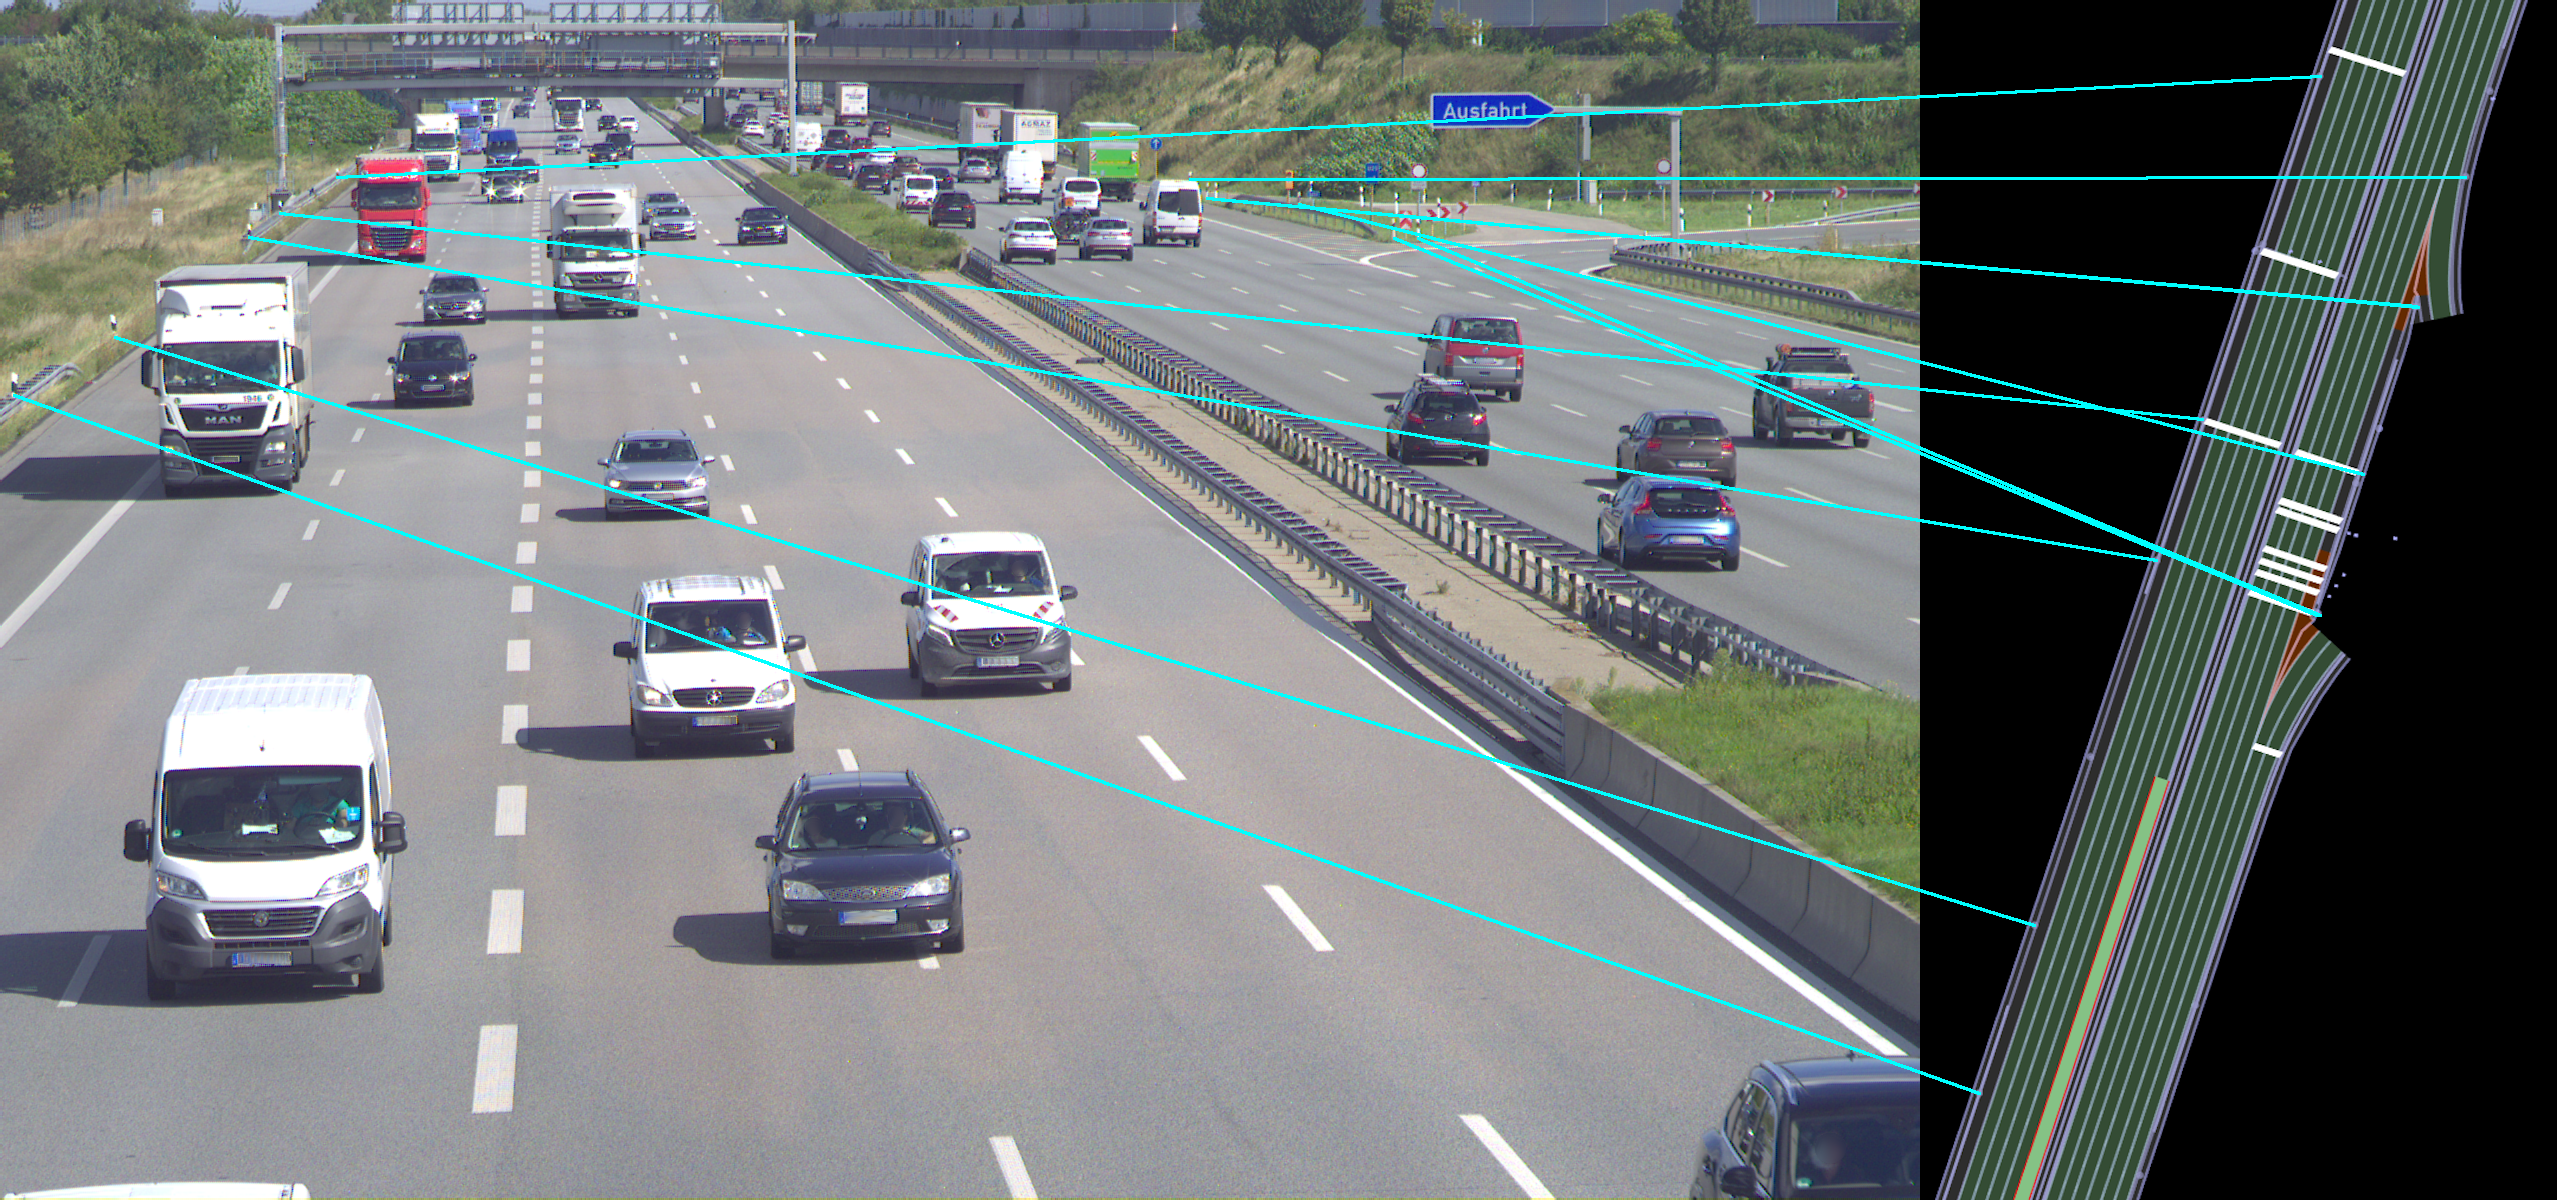
\includegraphics[width=\linewidth]{images/hd_map_mapping.png}
  \end{center}
     \caption{
       Left: The current camera frame. 
       Right: A part of the HD map.
       Light blue lines: An exemplary mapping $s_c \mapsto p_c$ from objects (right) to their corresponding pixels (left).
       }
  \label{fig:static_calibration_mapping}
  \end{figure}

We solve the BA problem by minimizing the reprojection-error over the PDs.
We thus require a set $C$ of correspondences that map world points $s_c$ of the PDs to their respective pixel $p_c$. 

This mapping is currently done by human interaction and not fully automated. 
We implemented an annotation tool to mark pixels that outputs a list of pixels that can easily be mapped to the list of objects.

%%%%%%%%%%%%%%%%%%%%%%%%%%%%%%%%%%%%%%%%%%%%%%%%%%%%%%%%%%%%%%%%%%%%%%%%%%%%%%%%%%%%%%%%%%%%%%%%%%%%%%%%%%%%%%%%%%%%%%%%%%%%%%%%%%%%%%%%%%%%%%%%%%%%%%%%%%%%%%%%%
%%%%%%%%%%%%%%%%%%%%%%%%%%%%%%%%%%%%%%%%%%%%%%%%%%%%%%%%%%%%%%%%%%%%%%%%%%%%%%%%%%%%%%%%%%%%%%%%%%%%%%%%%%%%%%%%%%%%%%%%%%%%%%%%%%%%%%%%%%%%%%%%%%%%%%%%%%%%%%%%%
%%%%%%%%%%%%%%%%%%%%%%%%%%%%%%%%%%%%%%%%%%%%%%%%%%%%%%%%%%%%%%%%%%%%%%%%%%%%%%%%%%%%%%%%%%%%%%%%%%%%%%%%%%%%%%%%%%%%%%%%%%%%%%%%%%%%%%%%%%%%%%%%%%%%%%%%%%%%%%%%%

\paragraph{Calibration procedure}
\begin{figure*}[!ht]
  \centering
  \begin{tabular}{cc}
    \includegraphics[width=0.4\linewidth]{images/calibration/background_uncalibrated_with_mapping.png}    &  
    \includegraphics[width=0.4\linewidth]{images/calibration/background_calibrated.png}    
  \end{tabular}
  \caption{Left: Sampled points of objects that are mapped to pixel locations (green) and sampled points without known corresponding pixels (red) rendered by a poorly calibrated camera model.
  The mapping from the points to their expected pixels is drawn in cyan.
  Right: The same sampled points after the calibration procedure.
  The rendered positions of the sampled points align with the pixels of the objects they are mapped to and the drawn mapping disappears as the distance approaches $0$.  }
  \label{fig:calibration}
  \end{figure*}

Our camera is modelled using the pinhole camera model. 
The pinhole projection from samples of the world objects to pixels is formulated as
\begin{equation}
  \label{eq:static_calibration_reprojection}
  p_c = \pi \left(  
    % \begin{bmatrix}
    %   R, T \\
    %   0, 1
    % \end{bmatrix} *
    R * T *
    (o_c + \lambda_c * h_c)
  \right)
\end{equation}
\begin{equation}
  \label{eq:static_calibration_intrinsic_parameters}
  z * \pi(x) =   
  \begin{bmatrix}
    f_x,& 0,& c_x,& 0\\
    0,& f_y,& c_y,& 0\\
    0,& s,& 1 ,& 0
  \end{bmatrix} * x 
\end{equation}
% \begin{equation}
%   \begin{bmatrix}
%     R, T \\
%     0, 1
%   \end{bmatrix} = 
%   \begin{bmatrix}
%     R, 0 \\
%     0, 1
%   \end{bmatrix} *
%   \begin{bmatrix}
%     0, T \\
%     0, 1
%   \end{bmatrix} =
%   R * T
% \end{equation}

where $R$ is the cameras world rotation in Euler angles, $T$ is the cameras world translation and $\pi$ is the camera projection to image space based on the camera intrinsic parameters.

The optimal value for $\pi,R,T$ is found, if it holds for all correspondences:
\begin{equation}
  0 = p_c - \pi \left( R * T * (o_c + \lambda_c * h_c)\right) = p_c - \hat{p}_c
\end{equation}

This places constraints on the values $\pi,R,T$ can take and enables us to recover the camera pose and intrinsics only from the correspondences.

We estimate the camera pose by minimizing a modified version of the least-squares reprojection error 
\begin{equation}
  \label{eq:static_calibration_error}
  \min_{T, R, \Lambda, W} E(P, S, \pi, T, R, \Lambda, W) 
\end{equation}
formulated as
\begin{equation}
  \begin{split}
  E(P, S, \pi, T, R, \Lambda, W ) =& 
  \sum_{c \in C} 
  \rho(\left\lVert 
    w_c * [ p_c - \hat{p}_c ]
  \right\rVert^2) \\ 
  +& 
  \sum_{c \in C} 
  \alpha * 
  \rho(\left\lVert 
  (1 - w_c)
  \right\rVert^2) \\ 
  +& 
  \sum_{c \in C} 
  \beta * 
  \rho(\left\lVert 
  \Delta(\lambda_c, 0, h_c)
  \right\rVert^2) \\ 
  +& 
  \sum_{\pi_i \in \pi} 
  \gamma *
  \rho(\left\lVert 
  \Delta (\pi_i, \pi_i * 0.9, \pi_i * 1.1)
  \right\rVert^2) \\
  +&
  \delta * 
  \rho(\left\lVert 
  \Delta (R_x, 60, 110)
  \right\rVert^2) \\
  +&
  \delta * 
  \rho(\left\lVert 
  \Delta (R_y, -10, 10)
  \right\rVert^2 
\end{split}
\label{eq:reprojection_error}
\end{equation}
where $P$ is the set of mapped pixels in the image, $S$ is the set of mapped corresponding sampled points from the objects and $\Lambda$ is the set of $\lambda$ values associated with the sampled points.
This formulation allows the optimization over the line approximations of the objects and jointly optimizes for the camera parameters $T, R$ and the $\lambda \in \Lambda$ parameters of the line objects.

The calculation of the exact position of $s_c \sim \lambda$ allows the optimizer to search the whole space of real numbers for $\lambda$.
Nonetheless we penalize values for $\lambda$ that exceed the physical height of the object by 
\begin{equation}
    \Delta (x, l, u) =
    \begin{cases}
      x - u,& \text{if } x > u\\
      x - l,& \text{if } x < l\\
      0,    & \text{else}
    \end{cases} 
\end{equation}
This regularization enables a robust estimation procedure that can flexibly adjust to the missing exact world positions.

\paragraph{Initialization}
In contrast to most pose estimation problems our approach drops the need for good initialization. 
By regularization of the $\lambda$ values enough flexibility is given to optimize over an infinite space of values, 
but enforces the solution of the $\lambda$ to lie within the interval of $\lambda \in [0, h]$.

\begin{equation}
  \bar{s} = \frac{1}{\left\lvert C \right\rvert } \sum_{c \in C} o_c 
\end{equation}

\begin{equation}
  T_0 = \begin{pmatrix}
    1, 0, 0,& \bar{s}_x \\   
    0, 1, 0,& \bar{s}_y \\   
    0, 0, 1,& \bar{s}_z + 1000 \\   
    0, 0, 0,& 1   
  \end{pmatrix}
\end{equation}

\begin{equation}
  R_0 = \mathbb{I} ^ {4 \times 4}
\end{equation}

It is sufficient to initialize with $\lambda_c = 0$ for all correspondences.
The camera rotation is defined to be zero with the camera facing in negative world $z$ axis.
By placing the camera at some distance over the mean of the known object positions with zero rotation the optimization always converges to the desired minimum.

% \begin{itemize}
%   \item HD map based approach
%   \item Optimization algorithm, reprojection error between map and video 
%   \item Landmark extraction, mapping, pose estimation
%   \item Watersheder for pixel marking
%  translation can be  and initializing the camera at the some distance over the mean    
 % \end{itemize}
% !TEX root=./report.tex

\section{Evaluation}

We assure the correctness and quantify the improvements resulting from the algorithms by an empirical study on the video streams of the highway cameras.

\subsection{Study Objects}
\begin{figure}[t]
    \begin{center}
    % \fbox{\rule{0pt}{2in} \rule{0.9\linewidth}{0pt}}
       \includegraphics[width=\linewidth]{images/cameras_schema.png}
    \end{center}
       \caption{The schematic camera setup along the highway A9.
       The cameras \camsf{4} and \camsn{4} are facing north,
       the cameras \camsf{5} and \camsn{5} are facing south.}
    \label{fig:cameras_schema}
    \end{figure}

We use video recordings from the four cameras mounted to the two gantry bridges internally named S40 and S50. The schematic camera setup is displayed in \autoref{fig:cameras_schema}.

The dataset consists of four recordings, each with of a length of $1495$ frames over $\sim 60$ seconds at $25$ frames per second.
The recordings are taken on a day with strong winds to ensure high jitter in the video feed to optimally test the dynamic stabilization pipeline described in \autoref{sec:dynamic_stabilization_approach}. 

%%%%%%%%%%%%%%%%%%%%%%%%%%%%%%%%%%%%%%%%%%%%%%%%%%%%%%%%%%%%%%%%%%%%%%%%%%%%%%%%%%%%%%%%%%%%%%%%%%%%%%%%%%%%%%%%%%%%
%%%%%%%%%%%%%%%%%%%%%%%%%%%%%%%%%%%%%%%%%%%%%%%%%%%%%%%%%%%%%%%%%%%%%%%%%%%%%%%%%%%%%%%%%%%%%%%%%%%%%%%%%%%%%%%%%%%%
%%%%%%%%%%%%%%%%%%%%%%%%%%%%%%%%%%%%%%%%%%%%%%%%%%%%%%%%%%%%%%%%%%%%%%%%%%%%%%%%%%%%%%%%%%%%%%%%%%%%%%%%%%%%%%%%%%%%

\subsection{Dynamic Stabilization}
\label{sec:evaluation_dynamic_stabilization}
We evaluate and compare three pipeline instances based on the SURF \cite{bay10.1007/11744023_32,opencv_library} feature detector (SURF), 
ORB \cite{rublee6126544, opencv_library} feature detector (ORB) and FAST \cite{Ghahremani_2021,opencv_library} feature detector with FREAK \cite{alahi6247715,opencv_library} feature descriptors (FAST) 
and present two metrics to evaluate the dynamic stabilization pipeline described in \autoref{sec:dynamic_stabilization_approach}.

%%%%%%%%%%%%%%%%%%%%%%%%%%%%%%%%%%%%%%%%%%%%%%%%%%%%%%%%%%%%%%%%%%%%%%%%%%%%%%%%%%%%%%%%%%%%%%%%%%%%%%%%%%%%%%%%%%%%
%%%%%%%%%%%%%%%%%%%%%%%%%%%%%%%%%%%%%%%%%%%%%%%%%%%%%%%%%%%%%%%%%%%%%%%%%%%%%%%%%%%%%%%%%%%%%%%%%%%%%%%%%%%%%%%%%%%%
%%%%%%%%%%%%%%%%%%%%%%%%%%%%%%%%%%%%%%%%%%%%%%%%%%%%%%%%%%%%%%%%%%%%%%%%%%%%%%%%%%%%%%%%%%%%%%%%%%%%%%%%%%%%%%%%%%%%

\subsubsection{Optical Flow}
\begin{figure*}[!ht]
    \centering
    \begin{tabular}{c}
      \includegraphics[width=0.95\linewidth]{images/frame_1317_cropped.png}    
    \end{tabular}
    \caption{
        From left to right: Original frame, stabilized using SURF, ORB and FAST.
        The dense optical flow displaying the pixel displacement, the lighter the color the further the displacement. 
        The angle of displacement is color coded according to the HSV color circle.  
        In the original frame the violet background color indicates a jittery camera movement. 
        The car in the lower half is driving in the opposite direction as the camera jitters. 
    }
    \label{fig:optical_flow_example}
\end{figure*}

The optical flow is a 2D vector field where each vector is a displacement vector showing the movement of points between frames caused by movement of the objects or cameras.
It describes the apparent motion of image objects between two consecutive frames. 

We use the dense optical flow estimation algorithm proposed by Farnebäck \cite{farnback10.1007/3-540-45103-X_50,opencv_library} to measure the displacement of each pixel between the frames. 
We calculate the mean displacement over the whole image to get the overall displacement. 

\autoref{fig:optical_flow_example} displays one frame of optical flow calculated pre and after stabilization.
It qualitatively shows that the static background scene is dark in the stabilized frames which indicates a low optical flow and thus nearly no movement. 
We see a car driving, indicated by the yellow patch, that remains as expected using SURF and ORB, but gets filtered out by FAST. This problem is described in \autoref{sec:dynamic_stabilization_evaluation_optical_flow_problem}.     

\begin{figure}[t]
    \centering
    \begin{tabular}{c}
      \includegraphics[width=0.9\linewidth]{diagrams/optical_flow/mean_pixel_shifts_after_dynamic_stabilization_s40_far.png}    \\  
      \includegraphics[width=0.9\linewidth]{diagrams/optical_flow/damping_mean_pixel_shifts_after_dynamic_stabilization_s40_far.png}    
\end{tabular}
    \caption{Top: 
        Comparison of the three implemented dynamic stabilizers (SURF, ORB, FAST) and the original not stabilized video feed using optical flow as metric (lower is better).
        The graphs display the mean pixel shift at each frame. 
        Bottom: 
        The damping capabilities of the same three stabilizers (higher is better). 
        The graphs approximate the removed jitter in the mean pixel shift between the original video and the stabilizer at each frame.\\
        For visualization the values are filtered using the rolling mean over 12 frames. 
        The light areas display the standard deviation within the window.
    }
    \label{fig:dynamic_stabilization_s40_far}
\end{figure}

\autoref{fig:dynamic_stabilization_s40_far} displays the mean pixel displacement (MPD) per frame calculated as the mean of the lengths of the vectors in the optical flow field and the damping as the difference of the mean displacements over the original and stabilized frame.
It shows that the original frames have a MPD of up to $5$ pixels per frame. This implies that on average every pixel on the dynamic scene and static background had moved by $5$ pixels per frame. 
The displacement is damped by all of the stabilizers by a mean of up to $4.5$ pixels, whereas the remaining displacement is due to the actually moving vehicles in the dynamic foreground.   

\begin{figure}[!ht]
      \includegraphics[width=\linewidth]{diagrams/optical_flow/stats.png}    
    \caption{
        Comparison of the percentages of more stable frames after dynamic stabilization per camera and stabilizer.
        A frame is classified as more stable if the MPD is lower than for the original video feed. 
    }
    \label{fig:dynamic_stabilization}
\end{figure}

\autoref{fig:dynamic_stabilization} displays the percentage of frames that are more stable than the original frame.
We define a frame to be more stable if its MPD is lower than the MPD of the original frame. 
It shows that for SURF and ORB at least $88.9\%$ ranging up to $99.7\%$ of frames are more stable.
For the FAST detector it shows that except for the \camsf{4} camera only between $67.2\%$ to $79.4\%$ of frames are more stable, whereas a value of $50\%$ would indicate that the other $50\%$ of frames are worse.  

\paragraph{Problem of optical flow as a metric}
\label{sec:dynamic_stabilization_evaluation_optical_flow_problem}
Unfortunately, optical flow exhibits one major problem as a metric: 
It cannot distinguish between dynamically moving objects and static scene.
This especially introduces a problem when a jitter of the camera moves the pixels in the same direction as the vehicles path is pointing in image space.
By this jitter the movement of the camera blurs the movement of the dynamic objects into the background and thus removes some of the real movement.
This shows some frames after stabilization to be worse than before. 
This should be taken with caution as the optical flow cannot detect the relative motion and thus is not a definite measure for the jitter.
Nonetheless it gives a good hint at the overall stabilization capabilities and can become a measure together with the following measure of the path length of a pixel on a dynamic object. 


%%%%%%%%%%%%%%%%%%%%%%%%%%%%%%%%%%%%%%%%%%%%%%%%%%%%%%%%%%%%%%%%%%%%%%%%%%%%%%%%%%%%%%%%%%%%%%%%%%%%%%%%%%%%%%%%%%%%
%%%%%%%%%%%%%%%%%%%%%%%%%%%%%%%%%%%%%%%%%%%%%%%%%%%%%%%%%%%%%%%%%%%%%%%%%%%%%%%%%%%%%%%%%%%%%%%%%%%%%%%%%%%%%%%%%%%%
%%%%%%%%%%%%%%%%%%%%%%%%%%%%%%%%%%%%%%%%%%%%%%%%%%%%%%%%%%%%%%%%%%%%%%%%%%%%%%%%%%%%%%%%%%%%%%%%%%%%%%%%%%%%%%%%%%%%


\subsubsection{Track features and calculate path smoothness}
To overcome the problems of the optical flow as a measure of stability we randomly took three sample vehicles per camera and tracked their pixel locations over time.
As the vehicles move the bounding box of the object is found using the Discriminative Correlation Filter With Channel and Spatial Reliability proposed by Lukezic \etal{} \cite{Lukezic_2017_CVPR,opencv_library}.
The middle point of the bounding box is then written to disk and used as the predicted pixel location of the object.

We only track in the original frame to remove inaccuracies in the tracking and use the homographic transformation matrix from \autoref{eq:homographic_transformation} that stabilizes the frame.
This gives us comparable results for the pixel locations. 

To calculate the arc length we use the sum of distances between the middle point pixel locations over frames. 
The middle point is formulated as 
\begin{equation}
    p = \begin{pmatrix}
        x + 0.5 * w \\
        y + 0.5 * h
    \end{pmatrix}
\end{equation}
with $x$ being the $x$-coordinate of the top left corner of the bounding box, 
$y$ being the $y$-coordinate of the top left corner of the bounding box, 
$w$ being the width of the bounding box and
$h$ being the height of the bounding box.

The arc length is described by
\begin{equation}
    arc(vehicle) = \sum_{n = 1}^{\left\lvert frames \right\rvert } \left\lVert 
        p_{i} - p_{i-1}
    \right\rVert _2
\end{equation} 

To get comparable results a normalization is performed by the arc length of the original video frame.
\begin{equation}
    narc_{stabilizer}(vehicle) = 
    \frac{arc_{stabilizer}(vehicle)}{arc_{original}(vehicle)}
\end{equation} 

\autoref{fig:object_tracking_s40_n_far} displays the vehicles tracked in the video sequence taken from the camera \camsn{4}. 
There is one red truck, a black pickup and a white car taken as a random sample.
The tracking is performed als long as they are visible.

As our dynamic stabilization algorithms remove environmental influences from the frames the pixels only move on the projected path of their vehicles.
\autoref{fig:object_tracking_s40_n_far} displays that the arc lengths after stabilization remain at only a relative length of $0.5$ of the original length.
This clearly indicates that with the same vehicle movement the tracked position is much more accurate.

\begin{figure*}[!ht]
    \centering
    \begin{tabular}{cc}
      \includegraphics[width=0.475\linewidth]{diagrams/object_tracking/s40_n_far/frame_cropped.png}    &  
      \includegraphics[width=0.475\linewidth]{diagrams/object_tracking/s40_n_far/arcs.png}    
\end{tabular}
    \caption{Left: 
    The exemplary vehicles tracked through the video sequence of the camera \camsn{4}. 
    Right:
    The corresponding normalized arc lengths of the pixel path. 
    The length is normalized by the original arc length, hence the 1.0 factor for the original video. 
    As the jitter is removed, the pixels movement is lowered significantly as it does only move with the vehicle, not the camera.
    This can be seen with around half of the path length remaining after stabilization for all stabilizers.
    }
    \label{fig:object_tracking_s40_n_far}
\end{figure*}

The 
\autoref{fig:object_tracking_appendix_s40_n_far}, 
\autoref{fig:object_tracking_appendix_s40_n_near}, 
\autoref{fig:object_tracking_appendix_s50_s_far} and 
\autoref{fig:object_tracking_appendix_s50_s_near} in \autoref{sec:appendix} display the tracked pixel locations of three cars per camera.

\subsubsection{Speed comparison}
% !TEX root=./report.tex

\subsection{Static calibration}
In the following we evaluate the implemented static calibration algorithm and assess the algorithmic and systematic errors.

\subsubsection{Ensure no Systematic Error}

\begin{figure*}[t]
    \centering
    \begin{tabular}{cc}
      \includegraphics[width=0.45 \linewidth]{images/calibration/google_maps_s50_s.png} &
      \includegraphics[width=0.45 \linewidth]{images/calibration/google_maps_s40_n.png} 
  \end{tabular}
  \caption{Left: The positions of the cameras \camsn{4} (red) and \camsf{4} (green) and their respective looking directions (yellow). 
  Right: The positions of the cameras \camsn{5} (red) and \camsf{5} (green) and their respective looking directions (yellow). 
  It displays that the rotation of the cameras is in a reasonable range so that the cameras look along the highway as expected. 
  Also the cameras are within reasonable translational bounds around their real world location as \autoref{sec:static_calibration_expectable_error} shows.
  }
  \label{fig:google_maps}
  \end{figure*}

The proposed pose estimation algorithm from \autoref{eq:static_calibration_error} converges to a pair of optimal translation $T$ and rotation $R$ values for the camera pose.
These $T, R$ values approximate the projection from the world objects to the pixels as described in \autoref{eq:static_calibration_reprojection}.

Using a maps provider we assured that the resulting values are within reasonable ranges and that there are no systematic errors in the optimization.
The results are displayed in \autoref{fig:google_maps}

\subsubsection{Points needed for convergence}
The correspondences build up a system of linear equations. 
This system of equations is solvable if there exist a more or equal number of constraints on the parameters than there are degrees of freedoms in the system:
\begin{equation}
  \label{eq:static_calibration_reprojection_evaluation}
  p_c = \pi \left(  
    % \begin{bmatrix}
    %   R, T \\
    %   0, 1
    % \end{bmatrix} *
    R * T *
    (o_c + \lambda_c * h_c)
  \right), \forall c \in C
\end{equation}
This is the case if:
\begin{equation}
  \begin{split}
  2 * \left\lvert C \right\rvert \quad \geq& \quad 5 + 3 + 3 + 1 * \left\lvert C \right\rvert \\
  \left\lvert C \right\rvert \quad \geq& \quad 11 
\end{split}
\end{equation} 

As each of the pixel per correspondence gives us two constraints and we optimize over the 5 intrinsic parameters (\autoref{eq:static_calibration_intrinsic_parameters}), the 3 extrinsic translation, 3 extrinsic rotation parameters and one $\lambda$ parameter per correspondence.
We see that 11 points are enough to recover the pose.

\subsubsection{Structure of points}
The best result are shown when there are at least two correspondences per object.
These correspondences should be the top and bottom most visible pixel of the object.
If there exists only 1 or a low number of near pixels, the algorithm cannot precisely recover the camera pose, as it is free to move the correspondence along the center line of the object.
The algorithm therefore cannot distinguish the solutions where the camera is placed low, thus projecting a high point of an object to a low pixel correspondence, 
or if it should place the camera higher and lower the correspondences world position along the center line.

We thus conclude that the best solution is recovered the more the pixels fill the whole object, and the more spread to the top and bottom of the object the correspondences are. 




























\subsubsection{Expectable Error Bounds}
\label{sec:static_calibration_expectable_error}

Due to measurement uncertainty in the camera sensors we expect some remaining error after pose estimation.
To conclude a lower bound on this error we start from the optimized focal length $f_px$ in pixels and the sensor width $w_{mm}$ in millimeters and $w_{px}$ in pixels.

The focal length in millimeters is given by 
\begin{equation}
  f_{mm} = f_{px} * \frac{w_{mm}}{w_{px}}
\end{equation}

We then calculate the field of view (FOV) in radians by 
\begin{equation}
  FOV_x = 2 * \arctan \left(\frac{f_{mm}}{2 * w_{mm}}\right)
\end{equation} 
Equivalent the $FOV_y$ with the height of the sensor $h_{mm}$.

This brings us to a formulation for the angle spanned by each pixel
\begin{equation}
  \alpha_{px} = \frac{w_{px}}{FOV_x}
\end{equation} 

Using the pythagorean formula we can then calculate the uncertainty $u$ in meters of the camera as the spanned meters per pixel relative to the distance $d$ from the camera 
\begin{equation}
  u = \tan (\alpha_{px}) * d
\end{equation}

\begin{table}
  \begin{center}
    \begin{tabular}{ |c | c | c| c| c| c |}
      \hline
      Camera & $f_{px}$ & $FOV_x [^{\circ}]$ & $\alpha_{px}$ & $d [m]$ & $u [cm]$ \\
      \hline
      \camsf{4} & 8591 & 12.753 & $1.16e^{-4}$ & 200 & 2.32 \\
      \camsf{4} & 8591 & 12.753 & $1.16e^{-4}$ & 650 & 7.54 \\
      \hline
      \camsn{4} & 2735 & 38.678 & $3.52e^{-4}$ & 25 & 0.88 \\
      \camsn{4} & 2735 & 38.678 & $3.52e^{-4}$ & 450 & 15.82 \\
      \hline
      \camsf{5} & 8868 & 12.357 & $1.12e^{-4}$ & 200 & 2.22 \\
      \camsf{5} & 8868 & 12.357 & $1.12e^{-4}$ & 650 & 7.30 \\
      \hline
      \camsn{5} & 2747 & 38.527 & $3.50e^{-4}$ & 25 & 0.88\\
      \camsn{5} & 2747 & 38.527 & $3.50e^{-4}$ & 450 & 15.76 \\
      \hline
    \end{tabular}
  \end{center}
  \caption{
    \label{tab:static_calibration_camera_uncertainty}
  }
\end{table}

\autoref{tab:static_calibration_camera_uncertainty} displays the uncertainty for our cameras.
It shows that the far cameras cannot distinguish between points that are $\sim 2.2 cm$ at the nearest visible distance from the camera ranging up to $\sim 7.54 cm$ at the farthest distance.
The near cameras cannot distinguish between points that are $\sim 0.88 cm$ at the nearest visible distance from the camera ranging up to $\sim 15.82 cm$ at the farthest distance.

This gives a lower bound for the uncertainty in the translational parameters of the camera.
The camera translation cannot be more precise as the lowest uncertainty in the measurements.
Nonetheless, in practice the error will sum up and the translation parameters will drift inevitable. 

This concludes that objects near to the camera are more reliable to detect and to use for estimation.





















\subsubsection{Expectable Deviations among Estimations}
The proposed pose estimation algorithm is based on the minimization of the reprojection-error \autoref{eq:static_calibration_reprojection}.
As with all optimization problems convergence is reached when the values that are optimized don't change anymore.

The optimization jointly optimizes for the 6 camera parameters, 3 for the translation, 3 for the Euler angle rotation and one $\lambda$ parameter per correspondence.
The resulting high-dimensional problem exceeds multiple minima, whereas each represents a configuration for the camera pose that well explains the dependency between pixels, world objects and the camera. 

As stated previously the loss landscape does exhibit a multitude of local minima, thus the optimization procedure converges to different sets of parameters. 

\begin{figure}[t]
  \centering
  \begin{tabular}{cc}
    \includegraphics[width=0.45 \linewidth]{diagrams/calibration/s40_n_far_small/parameters_all.csv/Translation[x]_vs_Loss[Correspondences]_vs_Loss[Lambdas]_cluster_All.png} &
    \includegraphics[width=0.45 \linewidth]{diagrams/calibration/s40_n_far_small/parameters_all.csv/Rotation[x]_vs_Loss[Correspondences]_vs_Loss[Lambdas]_cluster_All.png} \\
    
    \includegraphics[width=0.45 \linewidth]{diagrams/calibration/s40_n_far_small/parameters_all.csv/Translation[y]_vs_Loss[Correspondences]_vs_Loss[Lambdas]_cluster_All.png} &
    \includegraphics[width=0.45 \linewidth]{diagrams/calibration/s40_n_far_small/parameters_all.csv/Rotation[y]_vs_Loss[Correspondences]_vs_Loss[Lambdas]_cluster_All.png} \\
    
    \includegraphics[width=0.45 \linewidth]{diagrams/calibration/s40_n_far_small/parameters_all.csv/Translation[z]_vs_Loss[Correspondences]_vs_Loss[Lambdas]_cluster_All.png} &
    \includegraphics[width=0.45 \linewidth]{diagrams/calibration/s40_n_far_small/parameters_all.csv/Rotation[z]_vs_Loss[Correspondences]_vs_Loss[Lambdas]_cluster_All.png} \\
\end{tabular}
\caption{
  Left: The resulting translational parameters plotted against the remaining losses. 
  Right: The resulting rotational parameters plotted against the remaining losses.
  The mean of the distributions is displayed as thick dashed line. The smaller dashed lines display the standard deviation $\sigma$.
  The $\sigma$ of the translations does not exceed $2 * 10^{-4} m = 0.2 mm$.
  For the rotation $\sigma$ is at most $4 * 10^{-4} deg$.
  }
\label{fig:static_calibration_algorithmic_error}
\end{figure}

\autoref{fig:static_calibration_algorithmic_error} displays the resulting parameters for the camera \camsf{4}.
We plot the loss of the correspondence residuals and the $\lambda$ residual blocks against each of the parameters.
The translation parameters are in meters and relative to the transverse mercator projection \cite{lambert1894anmerkungen}.
The rotation parameters are in degree of Euler angles.

The plots show that the standard deviation $\sigma$ of the translations does not exceed $2 * 10^{-4} m = 0.2 mm$.
For the rotation $\sigma$ is at most $4 * 10^{-4} deg$. 

We have shown the expectable error for the parameters resulting from the sensor and map inaccuracies in \autoref{sec:static_calibration_expectable_error}. 
We conclude that in relation to these the algorithmic error can be neglected.

In the appendix \autoref{sec:appendix} we additionally evaluate the other cameras.

% \subsubsection{Minimal number of correspondences}

% !TEX root=./report.tex

\section{Future Work}
The project leaves us with the opportunities to research in a broad range of directions.

\subsection{Test on different weather/lighting conditions}
The implementations are currently only tested on good weather and lighting conditions. 
A next step is to test the implementations in bad weather and lighting conditions, \eg by night, rain and snow.
As far as we can tell by now the feature based dynamic stabilization approach will suffer in performance as the detected features will be compromised.
The static calibration nonetheless wont be impacted as we have the human-in-the-loop approach for correspondence mapping. 
When we switch to an automatic landmark detection algorithm the weather conditions will impact the detection and thus the calibration.

\subsection{Dynamic stabilization}
In the subfield of the dynamic stabilization we have until now implemented the visual feature based approach.

\subsubsection{Dropping stabilization if not enough correspondences found}
We showed in \autoref{sec:evaluation_dynamic_stabilization} that the number of better frames is not at 100\%.
This is partially due to the shortcomings of the optical flow used as a metric as described in \autoref{sec:evaluation_dynamic_stabilization_optical_flow_problem}.
Another problem arises when the feature matching does not give enough matches. 
Finding the homographic transformation is not well defined in this case anymore and the found solution can make the image stability worse.  

% \subsubsection{Dynamically pick best feature detector based on optical flow performance}
% Currently we empirically picked the SURF feature detector to have the best stabilization performance.
% We do measure the performance of the feature based dynamic stabilization approach based on the mean pixel deviation of the optical flow.
% As multiple feature detectors are already implemented together with the optical flow to measure the performance.
% To test would be to run all detectors in parallel and use the one with the most stabilize video output.

\subsubsection{Warp field stabilization based on Optical Flow}
Currently the optical flow is only used to measure performance but could be used as an alternative approach to the dynamic stabilization problem.
The optical flow is modelled as a vector field over the image and contains the pixel movement as direction vector and distance per pixel.
By inverting this vector field and thus applying the inverse of the jitter the image could be stabilized using image warping.  

\subsubsection{Deep Learning based approaches}
With the recent emerge of deep learning based approaches in computer vision, especially with convolutional neural networks (CNN), a self-learning stabilization procedure might be developed.
This might speed up the procedure and would inherently add a measure for the uncertainty of the results when finding the homographic transform.
Additionally the feature detection, matching and warping steps could be fused into one step and optimized jointly.

As far as we can tell this can be broken down into two approaches based on different loss functions.

\paragraph{Image MSE for calibration (unsupervised)}
Input the current frame and reference frame, output the homographic transformation. 
Learning is done by minimizing the mean squared error of pixel distances between the frames with the current transformation.

\paragraph{Logistic regression on pose (supervised)}
Input the current frame and reference frame, output the homographic transformation. 
Learning is done by logistic regression over the expected and predicted transform.

\subsection{Static calibration}
For the static calibration there are several improvements possible.

\subsubsection{IMU based sensor fusion}
Previous by-hand calibrations have shown that an inertia measurement unit (IMU) can be used to initially find a camera pose, but the lack of performance and huge time needed makes this not feasible.
This is just empirical knowledge, not backed up by research. 
This should be looked into further.

% \subsubsection{Extend to global refinement of multiple cameras}
% Currently the reprojection error as described in Eq. \ref{eq:reprojection_error} optimizes the pose of one camera \wrt the \HDmaps{}.
% By extending the optimization to jointly optimize over all cameras and their mappings a global calibration procedure can be established.
% The procedure might be formulated as
% formulated as
% \begin{equation}
%   \begin{split}
%   E(P, S, T, R, \Lambda, W ) =& 
%   \sum_{i \in Cams} \sum_{c \in C_i} 
%   \left\lVert 
%     w_c * [ p_{i,c} - \pi(T_i * R_i * s_c) ]
%   \right\rVert_2^2 \\ 
%   +& 
%   \sum_{i \in Cams} \sum_{c \in C_i} 
%   \left\lVert 
%   penalize(\lambda_c, h_c)
%   \right\rVert_2^2 \\ 
%   +& 
%   \sum_{i \in Cams} \sum_{c \in C_i} 
%   \left\lVert 
%   \alpha * (1 - w_c)
%   \right\rVert_2^2 
% \end{split}
% \label{eq:reprojection_error_global}
% \end{equation}
% where one should optimize over all cameras $i \in \text{Cameras}$ and the seen seen correspondences $c \in C_i$.
% This would finally give a per camera transformation $T_i$ and rotation $R_i$ that would be globally optimal also in relation to the other cameras.

\subsubsection{Automatic detection of more landmarks after initial calibration}
\label{sec:auto_detection_landmarks}
Currently the detection and mapping of landmarks is done by hand using a watershed algorithm \cite{meyer1992color,opencv_library} based external tool.
This tool relies on a by hand marking of landmarks as the markers used to find the segmentation.
By applying template, color or gradient matching approaches the detection of the markers might be automated.
This automated detection would speed up the mapping procedure. 

\subsubsection{Automatic mapping of pixels to objects}
\label{sec:auto_mapping_landmarks}
To establish the mapping of the correspondences a human has to look up the ids of the landmarks in the \HDmaps{}.
After an initial calibration an image region based approach might be used to automate this mapping.
This positions of the known objects from the \HDmaps{} can be projected into the camera image with the current camera pose.
Starting from the resulting pixel locations one could search in a defined enclosing region to search for pixels that clearly correspond to the objects.
This automatic detection of more landmarks could further improve the robustness an can be used to mitigate drift in the cameras.  

\subsubsection{Machine learning based pose estimation}
A machine learning based approach for the bundle adjustment problem we faced and the resulting camera pose estimation problem can be formulated.
As Aravkin \etal \cite{students_t_bundle_adjustment} have shown a Student's-t distribution based approach can be used to estimate and robustify the procedure against outliers.
  
\subsubsection{New HD map}
The newer OpenDRIVE standards also provide the possibility to include lane markings.
These lane markings are easily detectable and can then be used for the calibration procedure in conjunction with the object landmarks.
This would greatly simplify the automatic detection and mapping procedures as described in Sec. \ref{sec:auto_detection_landmarks} and Sec. \ref{sec:auto_mapping_landmarks} as they are spatially more extend and thus easier to detect.
Additionally with the color information, as the lane markings are always white (Germany) and yellow (USA) the detection is simplified a lot.
% !TEX root=./report.tex

\section{Conclusion}

In this paper we proposed two main improvements on the vision based tracking system used in the \Providentia{}.

We first presented a pipeline to dynamically stabilize jittery motion in the video streams of RGB cameras mounted to gantry bridges along a highway.
We applied a homographic transformation in image space based on the matching of visual features between the current and a stable reference frame.
We have shown that the stabilization substantially (up to $99.8\%$) improves the stability of the frames regarding the remaining mean pixel displacement.
By tracking vehicles through the video sequence we have shown that the remaining length of the pixels path after stabilization is as low as $43\%$ of the not stabilized one.
This implies that $57\%$ of the motion was noisy jitter that is removed after stabilization.
Finally, we have shown that the dynamic stabilization pipeline is easily realtime capable with at most $18.649$ milliseconds per frame.

We secondly presented the formulation of a single camera RGB-only Bundle Adjustment problem that is minimized using the reprojection-error.
We recover the cameras pose by jointly optimizing for the cameras intrinsic and extrinsic parameters as well as the real world position of viewed correspondences to a high definition map.
We checked our results for the absence of systematic errors, gave a lower bound on the number of correspondences needed for convergence and the structure the correspondences have to exceed.
We evaluated the expectable error after pose estimation that arises from measurement uncertainties and imprecisions in the HD map and have shown that the deviations among the minima found by the optimization strategy are neglectable.


\newpage
{
    \small
    \bibliographystyle{ieee_fullname}
    \bibliography{bib_literature}
}

% % !TEX root=./report.tex

\newpage

\section{Appendix}
\label{sec:appendix}
To declutter the report we moved many of the plots in this section.
Please see the next pages for the plots.

\begin{figure*}[!ht]
  \centering
    \begin{tabular}{cc}
      \includegraphics[width=0.475\linewidth]{diagrams/optical_flow/s40_n_far_image_raw.mp4.csv/compare_of_mean_pixel_displacement/window_size_12.html.png}    &  
      \includegraphics[width=0.475\linewidth]{diagrams/optical_flow/s40_n_far_image_raw.mp4.csv/deltas_of_mean_pixel_displacement/window_size_12.html.png}   \\ 

      \includegraphics[width=0.475\linewidth]{diagrams/optical_flow/s40_n_near_image_raw.mp4.csv/compare_of_mean_pixel_displacement/window_size_12.html.png}    & 
      \includegraphics[width=0.475\linewidth]{diagrams/optical_flow/s40_n_near_image_raw.mp4.csv/deltas_of_mean_pixel_displacement/window_size_12.html.png}   \\ 

      \includegraphics[width=0.475\linewidth]{diagrams/optical_flow/s50_s_far_image_raw.mp4.csv/compare_of_mean_pixel_displacement/window_size_12.html.png}    & 
      \includegraphics[width=0.475\linewidth]{diagrams/optical_flow/s50_s_far_image_raw.mp4.csv/deltas_of_mean_pixel_displacement/window_size_12.html.png}   \\ 

      \includegraphics[width=0.475\linewidth]{diagrams/optical_flow/s50_s_near_image_raw.mp4.csv/compare_of_mean_pixel_displacement/window_size_12.html.png}    &   
      \includegraphics[width=0.475\linewidth]{diagrams/optical_flow/s50_s_near_image_raw.mp4.csv/deltas_of_mean_pixel_displacement/window_size_12.html.png}   \\ 
    \end{tabular}
    \caption{
        Left: 
        The mean pixel shifts after stabilization with SURF, ORB and FAST compared to the original not stabilized video feed using optical flow as measure (lower is better).
        Right: 
        The damping of the mean pixel shifts of the same three stabilizers (higher is better). 
        The graphs approximate the removed jitter in the mean pixel shift between the original video and the stabilizers at each frame.\\
        For visualization the values are filtered using the rolling mean over 12 frames. 
        The light areas display the standard deviation within the window. \\
        It shows that for each of the stabilizers the damping is substantial, removes most of the jitter introduced by environmental influences and leaves only wanted movement of vehicles in the dynamic foreground.
    }
    \label{fig:dynamic_stabilization_appendix}
    \end{figure*}

    


\begin{figure*}[!ht]
  \centering
  \begin{tabular}{cc}
    \includegraphics[width=0.45\linewidth]{diagrams/object_tracking/s40_n_far/frame.png}    &  
    \includegraphics[width=0.475\linewidth]{diagrams/object_tracking/s40_n_far/normalized_arc_lengths.html.png}    \\

    \includegraphics[width=0.475\linewidth]{diagrams/object_tracking/s40_n_far/black_pickup.png}    &  
    \includegraphics[width=0.475\linewidth]{diagrams/object_tracking/s40_n_far/white_car.png}    \\  
    \includegraphics[width=0.475\linewidth]{diagrams/object_tracking/s40_n_far/red_truck.png}   
  \end{tabular}
  \caption{Top Left:
  The tracked vehicles in the camera \camsf{4} marked by their bounding boxes. 
  Top right: 
  The normalized arc lengths representing the path of the tracked pixels through the image.
  Bottom graphs:
  The tracked pixel locations of the vehicles as they move through the scene for the original video feed and the stabilized ones.
  The jittery motion of the camera can be clearly seen by the chaotic movement of the pixels.
  After stabilization the pixels move much more smoothly through the images, whereas the remaining jitter is mostly due to inaccuracies in the tracking. 
  }
  \label{fig:object_tracking_appendix_s40_n_far}
\end{figure*}



\begin{figure*}[!ht]
  \centering
  \begin{tabular}{cc}
    \includegraphics[width=0.45\linewidth]{diagrams/object_tracking/s40_n_near/frame.png}    &  
    \includegraphics[width=0.475\linewidth]{diagrams/object_tracking/s40_n_near/normalized_arc_lengths.html.png}    \\

    \includegraphics[width=0.475\linewidth]{diagrams/object_tracking/s40_n_near/black_car.png}    &  
    \includegraphics[width=0.475\linewidth]{diagrams/object_tracking/s40_n_near/silver_car.png}    \\  
    \includegraphics[width=0.475\linewidth]{diagrams/object_tracking/s40_n_near/white_truck.png}   
  \end{tabular}
  \caption{Top Left:
  The tracked vehicles in the camera \camsn{4} marked by their bounding boxes. 
  Top right: 
  The normalized arc lengths representing the path of the tracked pixels through the image.
  Bottom graphs:
  The tracked pixel locations of the vehicles as they move through the scene for the original video feed and the stabilized ones.
  It shows that the recording did not include much jitter and thus the paths are already relatively smooth.
   }
  \label{fig:object_tracking_appendix_s40_n_near}
\end{figure*}



\begin{figure*}[!ht]
  \centering
  \begin{tabular}{cc}
    \includegraphics[width=0.45\linewidth]{diagrams/object_tracking/s50_s_far/frame.png}    &  
    \includegraphics[width=0.475\linewidth]{diagrams/object_tracking/s50_s_far/normalized_arc_lengths.html.png}    \\

    \includegraphics[width=0.475\linewidth]{diagrams/object_tracking/s50_s_far/silver_car.png}    &  
    \includegraphics[width=0.475\linewidth]{diagrams/object_tracking/s50_s_far/white_truck.png}    \\  
    \includegraphics[width=0.475\linewidth]{diagrams/object_tracking/s50_s_far/yellow_truck.png}   
  \end{tabular}
  \caption{Top Left:
  The tracked vehicles in the camera \camsf{5} marked by their bounding boxes. 
  Top right: 
  The normalized arc lengths representing the path of the tracked pixels through the image.
  Bottom graphs:
  The tracked pixel locations of the vehicles as they move through the scene for the original video feed and the stabilized ones.
  The jittery motion of the camera can be clearly seen by the chaotic movement of the pixels.
  After stabilization the pixels move much more smoothly through the images, whereas the remaining jitter is mostly due to inaccuracies in the tracking. 
  The tracking of the silver car displays a lane change of the vehicle over two lanes.
  The tracking of the yellow truck displays an outlier for FAST as it extended the path of the tracked pixel.
  }
  \label{fig:object_tracking_appendix_s50_s_far}
\end{figure*}

\begin{figure*}[!ht]
  \centering
  \begin{tabular}{cc}
    \includegraphics[width=0.45\linewidth]{diagrams/object_tracking/s50_s_near/frame.png}    &  
    \includegraphics[width=0.475\linewidth]{diagrams/object_tracking/s50_s_near/normalized_arc_lengths.html.png}    \\

    \includegraphics[width=0.475\linewidth]{diagrams/object_tracking/s50_s_near/red_truck.png}    &  
    \includegraphics[width=0.475\linewidth]{diagrams/object_tracking/s50_s_near/red_van.png}    \\  
    \includegraphics[width=0.475\linewidth]{diagrams/object_tracking/s50_s_near/yellow_truck.png}   
  \end{tabular}
  \caption{Top Left:
  The tracked vehicles in the camera \camsn{5} marked by their bounding boxes. 
  Top right: 
  The normalized arc lengths representing the path of the tracked pixels through the image.
  Bottom graphs:
  The tracked pixel locations of the vehicles as they move through the scene for the original video feed and the stabilized ones.
  It shows that the recording did not include much jitter and thus the paths are already relatively smooth.
  }
  \label{fig:object_tracking_appendix_s50_s_near}
\end{figure*}

\begin{figure*}[!ht]
  \centering
  \begin{tabular}{cc}
    \includegraphics[width=0.45 \linewidth]{diagrams/calibration/s40_n_far/parameters.csv/Translation[x]_vs_Loss[Correspondences]_vs_Loss[Lambdas]_cluster_All.png} &
    \includegraphics[width=0.45 \linewidth]{diagrams/calibration/s40_n_far/parameters.csv/Rotation[x]_vs_Loss[Correspondences]_vs_Loss[Lambdas]_cluster_All.png} \\
    
    \includegraphics[width=0.45 \linewidth]{diagrams/calibration/s40_n_far/parameters.csv/Translation[y]_vs_Loss[Correspondences]_vs_Loss[Lambdas]_cluster_All.png} &
    \includegraphics[width=0.45 \linewidth]{diagrams/calibration/s40_n_far/parameters.csv/Rotation[y]_vs_Loss[Correspondences]_vs_Loss[Lambdas]_cluster_All.png} \\
    
    \includegraphics[width=0.45 \linewidth]{diagrams/calibration/s40_n_far/parameters.csv/Translation[z]_vs_Loss[Correspondences]_vs_Loss[Lambdas]_cluster_All.png} &
    \includegraphics[width=0.45 \linewidth]{diagrams/calibration/s40_n_far/parameters.csv/Rotation[z]_vs_Loss[Correspondences]_vs_Loss[Lambdas]_cluster_All.png} \\

    \includegraphics[width=0.45 \linewidth]{diagrams/calibration/s40_n_far/parameters.csv/FocalLength_vs_Loss[Correspondences]_vs_Loss[Lambdas]_cluster_All.png} &
\end{tabular}
\caption{
  Camera: \camsf{4}.
  Left: The resulting translational parameters plotted against the remaining losses. 
  Right: The resulting rotational parameters plotted against the remaining losses.
  Bottom: The resulting focal length  plotted against the remaining losses.
   }
\label{fig:static_calibration_algorithmic_error_s40_n_far}
\end{figure*}

\begin{figure*}[!ht]
  \centering
  \begin{tabular}{cc}
    \includegraphics[width=0.45 \linewidth]{diagrams/calibration/s40_n_near/parameters.csv/Translation[x]_vs_Loss[Correspondences]_vs_Loss[Lambdas]_cluster_All.png} &
    \includegraphics[width=0.45 \linewidth]{diagrams/calibration/s40_n_near/parameters.csv/Rotation[x]_vs_Loss[Correspondences]_vs_Loss[Lambdas]_cluster_All.png} \\
    
    \includegraphics[width=0.45 \linewidth]{diagrams/calibration/s40_n_near/parameters.csv/Translation[y]_vs_Loss[Correspondences]_vs_Loss[Lambdas]_cluster_All.png} &
    \includegraphics[width=0.45 \linewidth]{diagrams/calibration/s40_n_near/parameters.csv/Rotation[y]_vs_Loss[Correspondences]_vs_Loss[Lambdas]_cluster_All.png} \\
    
    \includegraphics[width=0.45 \linewidth]{diagrams/calibration/s40_n_near/parameters.csv/Translation[z]_vs_Loss[Correspondences]_vs_Loss[Lambdas]_cluster_All.png} &
    \includegraphics[width=0.45 \linewidth]{diagrams/calibration/s40_n_near/parameters.csv/Rotation[z]_vs_Loss[Correspondences]_vs_Loss[Lambdas]_cluster_All.png} \\

    \includegraphics[width=0.45 \linewidth]{diagrams/calibration/s40_n_near/parameters.csv/FocalLength_vs_Loss[Correspondences]_vs_Loss[Lambdas]_cluster_All.png} &
\end{tabular}
\caption{
  Camera: \camsn{4}.
  Left: The resulting translational parameters plotted against the remaining losses. 
  Right: The resulting rotational parameters plotted against the remaining losses.
  Bottom: The resulting focal length  plotted against the remaining losses.
     }
\label{fig:static_calibration_algorithmic_error_s40_n_near}
\end{figure*}

\begin{figure*}[!ht]
  \centering
  \begin{tabular}{cc}
    \includegraphics[width=0.45 \linewidth]{diagrams/calibration/s50_s_far/parameters.csv/Translation[x]_vs_Loss[Correspondences]_vs_Loss[Lambdas]_cluster_All.png} &
    \includegraphics[width=0.45 \linewidth]{diagrams/calibration/s50_s_far/parameters.csv/Rotation[x]_vs_Loss[Correspondences]_vs_Loss[Lambdas]_cluster_All.png} \\
    
    \includegraphics[width=0.45 \linewidth]{diagrams/calibration/s50_s_far/parameters.csv/Translation[y]_vs_Loss[Correspondences]_vs_Loss[Lambdas]_cluster_All.png} &
    \includegraphics[width=0.45 \linewidth]{diagrams/calibration/s50_s_far/parameters.csv/Rotation[y]_vs_Loss[Correspondences]_vs_Loss[Lambdas]_cluster_All.png} \\
    
    \includegraphics[width=0.45 \linewidth]{diagrams/calibration/s50_s_far/parameters.csv/Translation[z]_vs_Loss[Correspondences]_vs_Loss[Lambdas]_cluster_All.png} &
    \includegraphics[width=0.45 \linewidth]{diagrams/calibration/s50_s_far/parameters.csv/Rotation[z]_vs_Loss[Correspondences]_vs_Loss[Lambdas]_cluster_All.png} \\

    \includegraphics[width=0.45 \linewidth]{diagrams/calibration/s50_s_far/parameters.csv/FocalLength_vs_Loss[Correspondences]_vs_Loss[Lambdas]_cluster_All.png} &

  \end{tabular}
\caption{
  Camera: \camsf{5}.
  Left: The resulting translational parameters plotted against the remaining losses. 
  Right: The resulting rotational parameters plotted against the remaining losses.
  Bottom: The resulting focal length  plotted against the remaining losses.
    }
\label{fig:static_calibration_algorithmic_error_s50_s_far}
\end{figure*}

\begin{figure*}[!ht]
  \centering
  \begin{tabular}{cc}
    \includegraphics[width=0.45 \linewidth]{diagrams/calibration/s50_s_near/parameters.csv/Translation[x]_vs_Loss[Correspondences]_vs_Loss[Lambdas]_cluster_All.png} &
    \includegraphics[width=0.45 \linewidth]{diagrams/calibration/s50_s_near/parameters.csv/Rotation[x]_vs_Loss[Correspondences]_vs_Loss[Lambdas]_cluster_All.png} \\
    
    \includegraphics[width=0.45 \linewidth]{diagrams/calibration/s50_s_near/parameters.csv/Translation[y]_vs_Loss[Correspondences]_vs_Loss[Lambdas]_cluster_All.png} &
    \includegraphics[width=0.45 \linewidth]{diagrams/calibration/s50_s_near/parameters.csv/Rotation[y]_vs_Loss[Correspondences]_vs_Loss[Lambdas]_cluster_All.png} \\
    
    \includegraphics[width=0.45 \linewidth]{diagrams/calibration/s50_s_near/parameters.csv/Translation[z]_vs_Loss[Correspondences]_vs_Loss[Lambdas]_cluster_All.png} &
    \includegraphics[width=0.45 \linewidth]{diagrams/calibration/s50_s_near/parameters.csv/Rotation[z]_vs_Loss[Correspondences]_vs_Loss[Lambdas]_cluster_All.png} \\

    \includegraphics[width=0.45 \linewidth]{diagrams/calibration/s50_s_near/parameters.csv/FocalLength_vs_Loss[Correspondences]_vs_Loss[Lambdas]_cluster_All.png} &
\end{tabular}
\caption{
  Camera: \camsn{5}.
  Left: The resulting translational parameters plotted against the remaining losses. 
  Right: The resulting rotational parameters plotted against the remaining losses.
  Bottom: The resulting focal length  plotted against the remaining losses.
     }
\label{fig:static_calibration_algorithmic_error_s50_s_near}
\end{figure*}



\end{document}
